\externaldocument{modelling}

\section{Experiments and Results}
For all the plots of the experiments the red curve indicates the tumour cell density, the blue curve the ECM density and the green curve the MDE concentration. In all of the experiments we used the value of $\epsilon = 0.01$ to match the inital conditions from \cite{anderson_mathematical_2000} and \cite{Kolev2010}. \newline 
Mathematical Intuition of the three curves and how the parameters interact.


\subsection{Two dimensional Results without Proliferation}
\subsubsection{Replicating results}
We will start with replicating previous results from Anderson et al.\cite{anderson_mathematical_2000}, Figure 1, making our curves fit the findings in their diagramms. 

%naming convention of figures: d0_d1_d2_eta_alpha_beta_gamma_mu1_mu2

\begin{figure}[t]
    \centering
    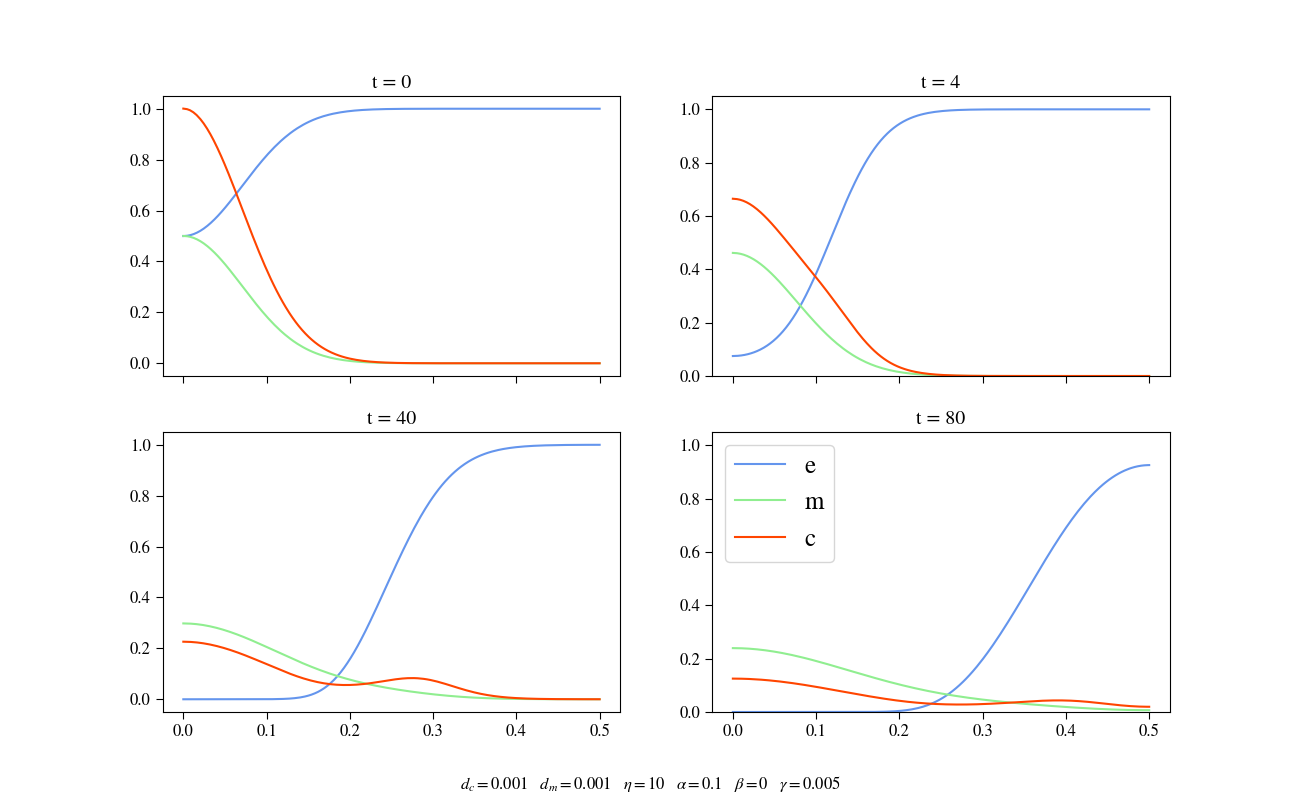
\includegraphics[width=\textwidth]{resources/images/2D_1e-3_1e-3_1e-3_10_0.1_0_0.005_1e-2_10_plot.png}
    \caption{Caption}
    \label{fig:2D_1e-3_1e-3_1e-3_10_0.1_0_0.005}
\end{figure}
In the first simulation the same parameter were used as in Anderson et al. first one dimensional experiment; $d_c = 0.001, d_m = 0.001, \gamma = 0.005, \eta = 10, \alpha = 0.1, \beta = 0, \mu_1 = 0, \mu_2 = 0$. Figure~\ref{fig:2D_1e-3_1e-3_1e-3_10_0.1_0_0.005} shows 4 snapshots of different points in time of tumour cell density, extracellular matrix density and matrix degrading enzymes concentration. In the conducted experiments it was shown that for every step in time done in the original paper we have done 4 steps, this is the reason for our time scale. Starting from the inital values seen at $t=0$ we see that after four time steps a very small unevenness has formed for the tumour cell density at $x\approx 0.1$. Both concentrations of MDEs and ECM have decreased as expected, looking at the model, MDEs have also invaded into the surrouding tissue, stretching the initial concentration around the origin.
In the next image showing the simulation after 40 timesteps we see that this unevenness has been propagated to form a hill at the leading edge of the tumour cells invading the surrounding tissue, at $x\approx 0.28$. MDEs also continued their diffusion into the area, decaying the ECM in their wake, decreasing them further. 
The last image, after 80 simulation time steps, we see that as well the hill that has formed at the leading edge of the tumour cells as well as the concentration of tumour cells at the origin, has decreased, due to the diffusion factor and the haptotactic flux. If we were to look at the simulation at later points in time, this curve will flatten even more, since with more time the ECM will be decayed and therefore the haptotactic flux coefficient $\gamma$ will lose its influence, leaving the movement of the cells to diffusion only. The curve for the MDEs has also flattened, yet not as strongly as the tumour cells concentration and as the observed before the ECM decayed where the MDEs were previously.\newline
Comparing \ref{fig:2D_1e-3_1e-3_1e-3_10_0.1_0_0.005} to figure 1 in \cite{anderson_mathematical_2000}, we can see major differences. The first image showing $t=0$ looks the same, which confirms that both experiments start with the same initial values. In the images showing the simulation at the second time checkpoint we see that though the tumour concentration and ECM density values are approximately the same, the MDE concentration is slightly lower in our experiment, which will get more pregnant in the later images. The unevenness having formed at the leading edge of the tumour cell concentration also looks to be slightly smaller. The differences in the third image are more strikingly, both $c$ and $m$ have considerably lower concentrations, yet the ECM value looks to in line. In our case the diffusion of the tumour cells into the tissue also seems to happen a littel bit too fast. The last time checkpoints manifest our findings, showing the same behaviour with ECM being approximately the same, tumour cell density and MDE concentration being clearly lower in our experiment and invasion of tissue happening too fast, leaving the lump at the origin $x=0$ too small. \newline 
This first of all confirms the initial supposition that with changing the dimension for the simulations the results also vary. We will now adjust the parameters iteratively to align our results with above compared experiment. For this we will now start with varying the MDE production coefficient $\alpha$, to get higher concentration values, and also change the diffusion terms $d_c$ and $d_m$, to adjust the pace of the invasion of tumour cells and MDEs into the area.

\begin{figure}[h]
    \centering
    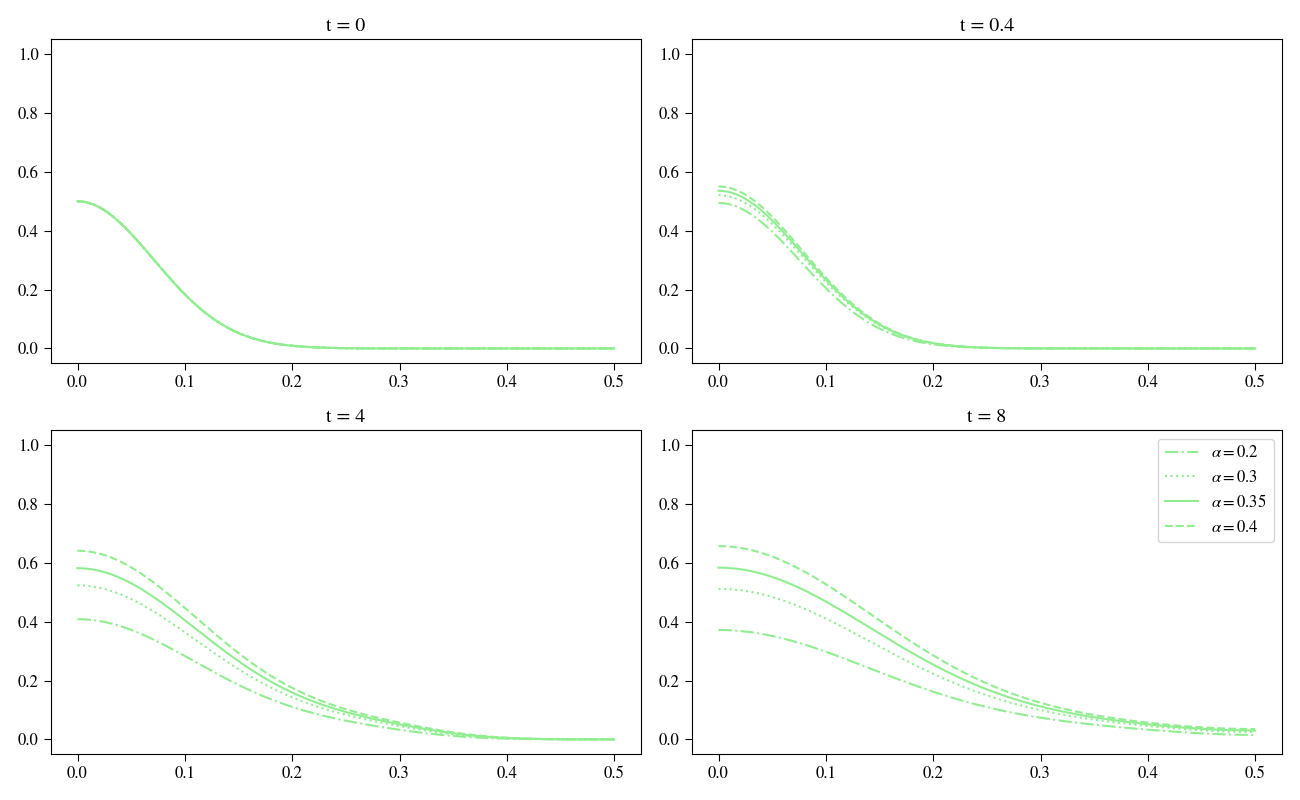
\includegraphics[width=\textwidth]{resources/images/alpha_comparison.png}
    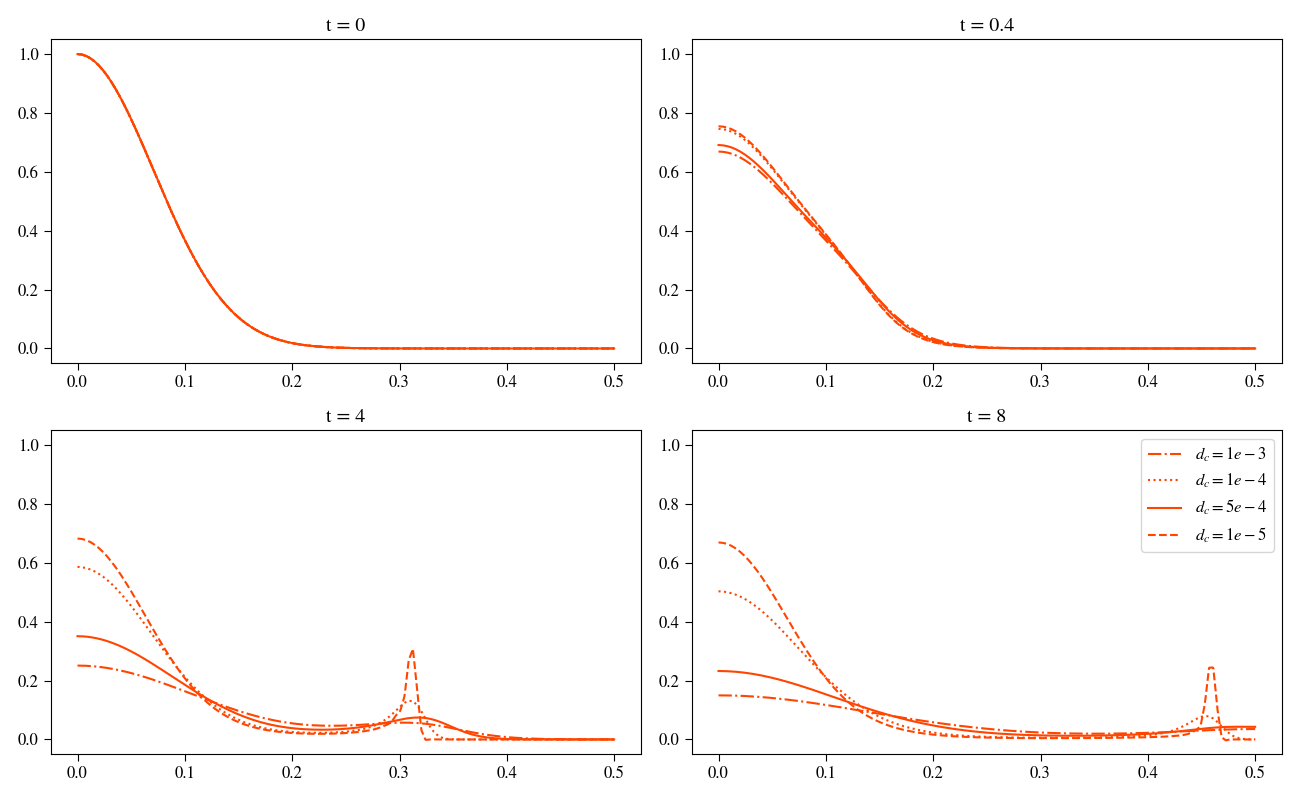
\includegraphics[width=\textwidth]{resources/images/dc_comparison.png}
    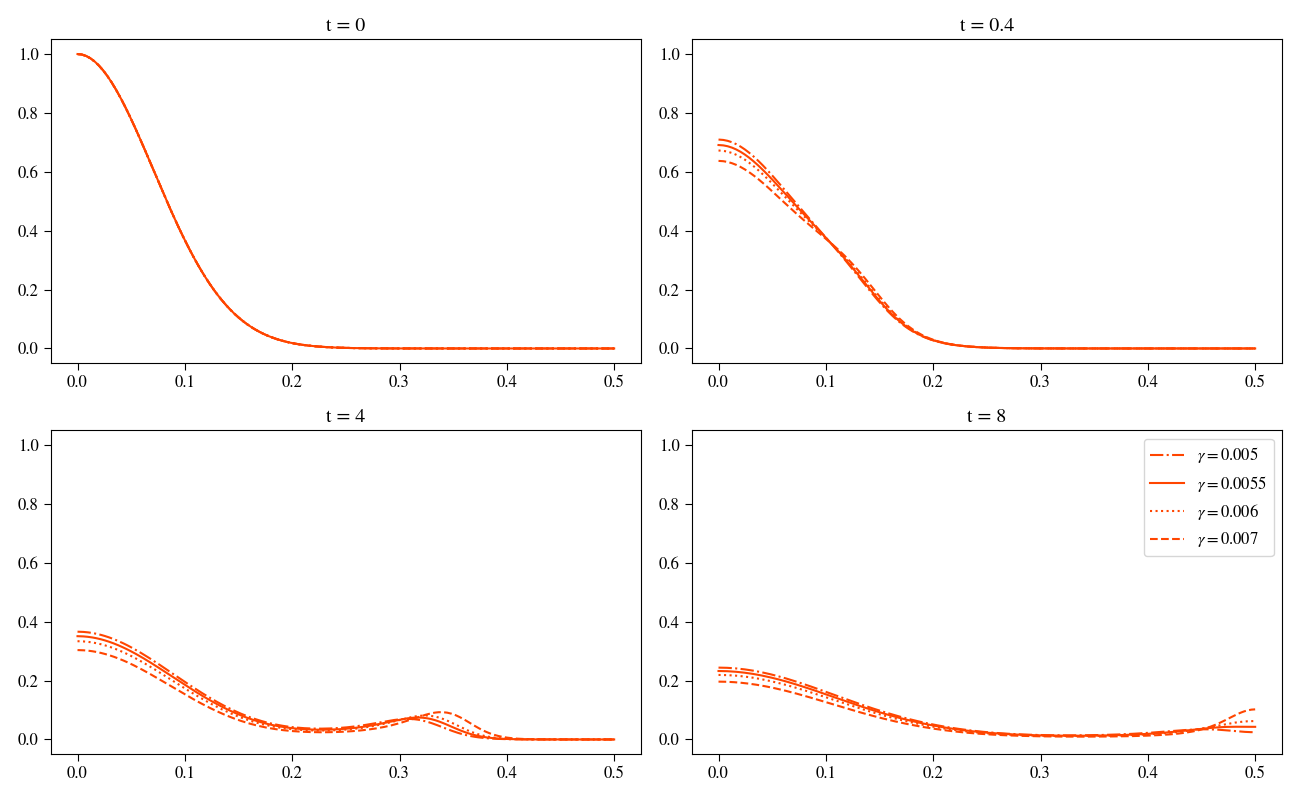
\includegraphics[width=\textwidth]{resources/images/gamma_comparison.png}
    \caption{Caption}
    \label{fig:replication_comparison}
\end{figure}
Figure~\ref{fig:replication_comparison} shows a comparison of the parameters $\alpha$, $d_c$ and $\gamma$ have on a specific curve. Comparing different values for $\alpha$ and their effect on the curve of the MDE concentration, shows that, especially looking at the later points in time $t=4$ and $t=8$, with values for $\alpha$ between $0.3$ and $0.4$ we will get a good approximation. The values of the original paper for the MDEs are for $t=4$ $m(0)=0.6$ and at $t=8$ $m(0)=0.7$. Fine tuning this parameter led us to $\alpha=0.35645$.\newline 
Looking at $d_c$ we chose a value of $d_c=5e-4$. Using higher values for this parameter will result in numerical instability and results that are not useable. For $\gamma$ we made a slight adjustment upwards to $\gamma=0.0055$ to have a little bit more pull on the tumour cells outward, to match the invasion speed observed in the original paper. This yields results where the small hill at the leading edge of the tumour cell concentration in the latter two points in time is a higher values for $x$, yet not as steep as for example $\gamma = 0.007$. \newline 
\begin{figure}[t]
    \centering
    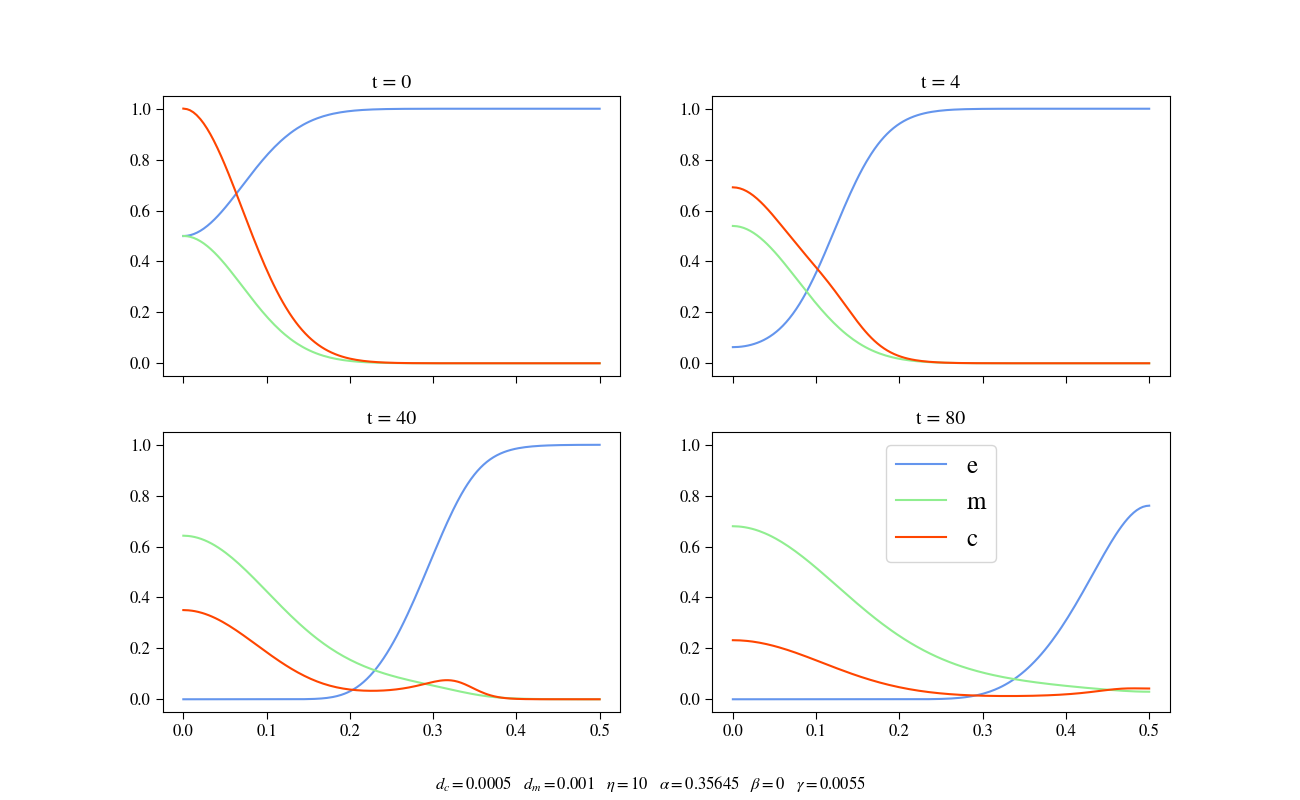
\includegraphics[width=\textwidth]{resources/images/2D_5e-4_1e-3_1e-3_10_0.35645_0_0.0055_1e-2_10_plot.png}
    \caption{Caption}
    \label{fig:2D_5e-4_1e-3_1e-3_10_0.35645_0_0.0055}
\end{figure}
These adjustments leave with the final configuration for replicating the system with the curves in figure~\ref{fig:2D_5e-4_1e-3_1e-3_10_0.35645_0_0.0055} and the parameter settings also seen in the same figure.
Slightly adjusting the haptotatic flux to $\gamma=0.0055$ yields the following results, seen in figure~\ref{fig:2D_5e-4_1e-3_1e-3_10_0.35645_0_0.0055}. comparing our final version with the original one we can see that in the second point in time, at $t=4$ in our case, the values of the three curves at the $x=0$ are nearly the same. In the original experiment the bump in the curve for the tumour concentration looks more pregnant, but this is only due to the fact, that this experiment was most likely done on the unit line, not the unit cube, and therefore the x-scale has been streched to $y_{max}=1$ where in our case it is $x_{max} = 0.5$. The two later points in time confirm the similarity with having also nealy the same values for the three curves at $x=0$ but also their respective propagations in time look to be in line with the original experiment. 



\subsubsection{Parameter Analysis}
From the replicated results shown in figures~\ref{fig:2D_5e-4_1e-3_1e-3_10_0.35645_0_0.0055}, we saw that if we variate certain parameters the results also vary strongly. Therefore we are now going to have a look at how changing one parameter affects the output of the whole system. For this we assume the parameter values of the replicated results to be our set of baseline parameters, from there in each experiment only one parameter is changed. 
\subsubsection*{$d_c$ Variation}ersetzen
The parameter analysed in this section describes the diffusion of the tumour cells and is integrated into the equations as being dependent on the laplacian of the tumour cells $\Delta c = (\frac{\partial c}{\partial x} + \frac{\partial c}{\partial y} + \frac{\partial c}{\partial z})$. Leaving out the proliferation term our equation for $\frac{\partial c}{\partial t}$ also depends on $\gamma$ a coefficient for the haptotatic flux. The mathematical intuition is that if we will decrease $d_c$ we will see the effects of $\gamma$ taking over the simulation results for the $c$ curve, meaning that the tumour cells are more likely to drift outward and let themselves be pulled by the ECM concentration $e$, leaving ony a little concentration at the origin, creating a bigger hill on the leading edge of the tumour concentration, below where $c \nabla e$ will be highest. On the other hand if we increase $d_c$ the effects of haptotaxis will diminish, the tumour cells will be subject to bigger diffusion pulling them more evenly into the tissue, there will be no leading hill being pulled outwards, since the diffusion will happen too fast, making this effect irrelevant. 
\begin{figure}[h]
    \centering
    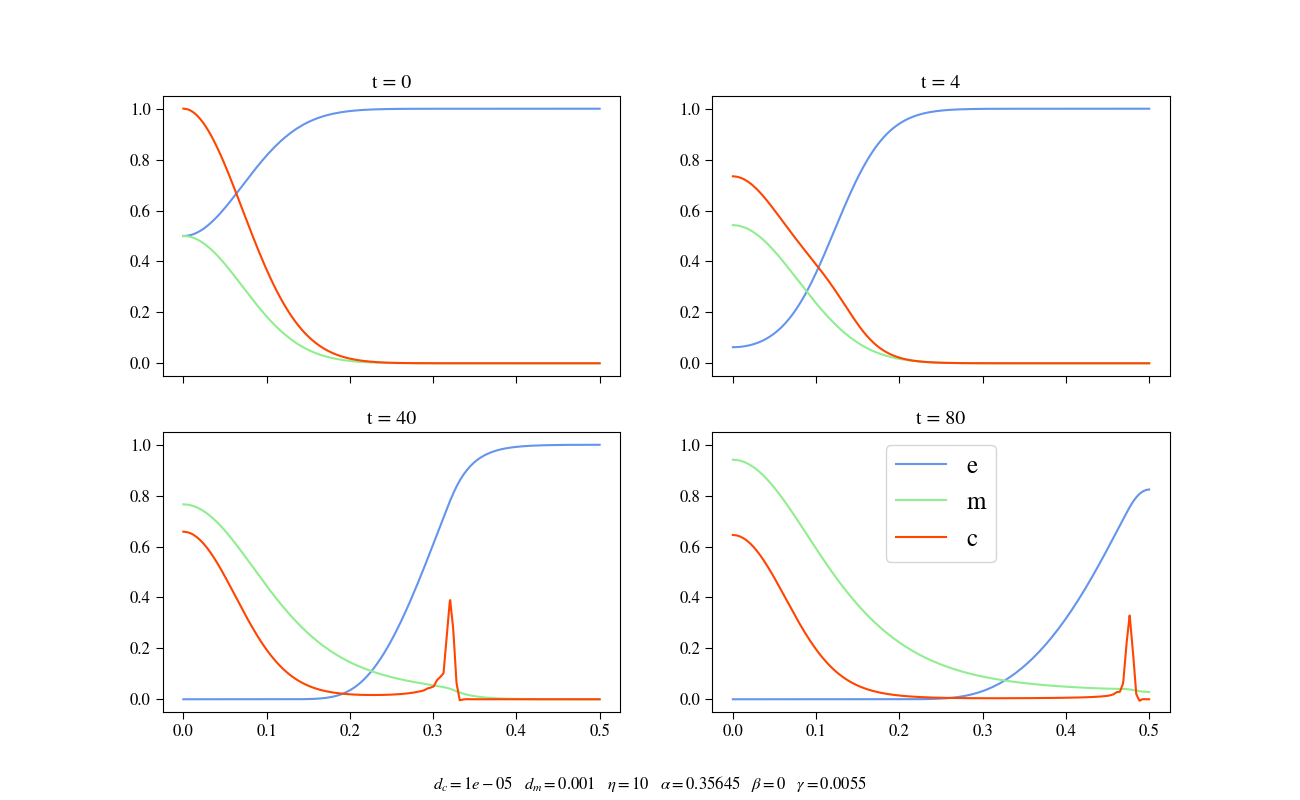
\includegraphics[width=\textwidth]{resources/images/2D_10e-6_1e-3_1e-3_10_0.35645_0_0.0055_1e-2_10_plot.png}
    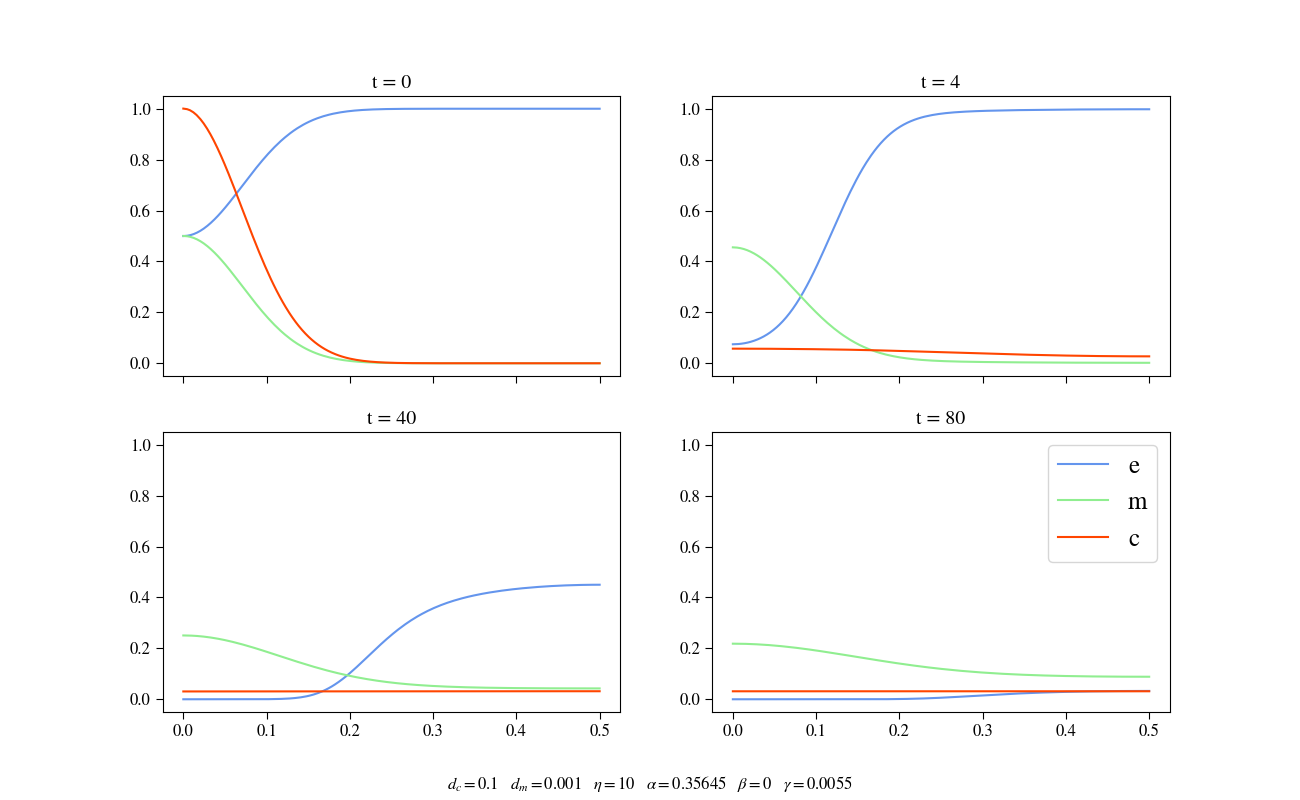
\includegraphics[width=\textwidth]{resources/images/2D_1e-1_1e-3_1e-3_10_0.35645_0_0.0055_1e-2_10_plot.png}
    \caption{Caption}
    \label{fig:dc_comparison}
\end{figure}

Looking at both experiments in figure~\ref{fig:dc_comparison}, we can see these assumptions confirmed. The smaller $d_c$ gets the higher the influence of $\gamma$ will be and vice versa. In the first four images we can see the results for $d_c=1e-5=0.00005$, while in the it looks mostly normal with little of the secession building at the leading edge, we can see that in the third image, this secession has not only seperated itself from the main lump of cells, but has also developed a sharp peak, which would have negative consequence regarding the differentiability of the $c$ curve. In the fourth image this behaviour is even more extreme and looking closely at this simulation in ParaView, the values for $c$ take on a negative sign, which from a biological perspective does not make any sense since there can't be less than zero cells at a position in space. This indicates a numerical instability, which decreasing $d_c$ even furhter also resulted in oscilations in the $c$ curve and even more negative values for the tumour cells. This instability is due to numercial model used, which only yields useful results if $\gamma$ and $d_c$ are in a certain range. This could be a point for further investigation, inspecting how the results change if $\gamma$ and $d_c$ are both varied at the same time and finding this range $\gamma$ and $d_c$ need to be in to make sense. However looking at the other two curves $e$ and $m$ we can see that they still make sense, especially also in the first experiment with $d_c=1e-5$, $m$ at the start following where $c$ was high, exceeding $c$ at some point due to the production factor $\alpha$ and $e$ decaying where the MDEs have higher values. Interesting is that having high values for the diffusion coefficient the concentration is faster evenly distributed in space, which indicates a higher invasion pace, which in turn makes the degradation of $e$ happen a lot faster, though the MDEs have taken on a near constant niveau throughout space. This also indicates, that we don't need to have a visibly higher concentration of $m$ to degrade the ECM. 

\subsubsection*{$\gamma$ Variation}
Inspecting the effects of $\gamma$ we can assume the same as for $d_c$ if we select higher values for $\gamma$ the effects of haptotaxis, pulling the tumour cells into the tissue faster, leaving no cells at the origin, taking lower values for $\gamma$, the diffusion will be superior factor for the tumour cell motility, which will result in no secession at the leading edge of the tumour cells.

The experiments verify this behaviour, in the first one where $\gamma=0.002$ we can see the effects of haptotaxis only slightly in the third image, with a small bump for the tumour cells the farthest out. Increasing $\gamma=0.008$ we see the haptotatic effects stronger now than in the base case, the secession that gets pulled into the tissue is getting bigger and also the invasion pace at which tumour cells reach the outer regions is faster. Selecting even higher values as $\gamma = 0.01$ we see this behaviour increasing the secession at the leading edge of the tumour cells is now almost as big as the remaining part at the origin, the invasion pace and therefore also the degradation of the ECM is accellerated. When we now take a step further and increase $\gamma$ by one potence, we can observe that the invasion pace, has gotten so high, that before finishing the simulation at $t=8$ the tumour cells have not only invaded completely up to the border but have also been pulled back towards the origin upon getting reflected at the border of the unit square and also since degradation of the ECM has not kept up with the tumour cells, leaving a situation where the tumour cells have spread further than the ECM and are now being pulled backwards again. This is therefore the first experiment which has in eight times produced results that are not longer resemble radial symmetry as seen in image ..., where we can see that the diffusion and haptotaxis properties of the tumour cells push them into the corners of the unit square, where there is still the highest concentration of ECM and afterwards back in from corners again due to haptotaxis.
Taking a look at the other curves we also get interesting results, as expected when we decrease $\gamma$ and let $d_c$ stay constant the invasion pace will decrease, having also degraded the ECM in the outer regions than the base case and also having higher MDE concentrations towards the origin since it stayed longer in these regions during the experiment. Increasing $\gamma$ over the value of the base case resulted also in hihger invasion pace, ECM degradation and lower MDE values at the origin, but this behaviour does not increase linearly. Looking at the experiment with $\gamma=0.1$ we see that though the tumour cells have reached the border regions faster, the ECM degradation could not keep up with the pace, resulting in areas where the ECM is still high, the tumour cells have already surpassed, but have not produced enough MDEs to degrade it. Where in all of the other experiments the tumour cells invaded at such a pace, that the produced MDEs in their wake were sufficient to degrade the ECMs to not pull the tumour cells back to the remaining ECMs later. This is also only experiment where the MDe curve $m$ is not monotone decreasing, with higher values at the origin and bordering regions, but lower one in between. If we were to increase $\gamma$ further we would see this behaviour mirrored, with the tumour cells spreading so fast throughout the space that we would get oscilations.

$\textcolor{red}{insert 2D image since now it depends on the cube not anymore radially symmetrical also new time stamps for observing effects}$

\subsubsection*{$\eta$ Variation}
The parameter $\eta$ only directly influences the degrading of the ECM, which happens faster for higher $\eta$ coefficients in regions where both MDE and ECM concentration are high. Varying this parameter yet may have a high impact of the solution because, the gradient of the ECM is a deciding factor for the effects of haptotaxis on the tumour cells. \newline
The first experiment in figure .. shows that if $\eta = 0$, which means that the ECM is not degraded by the MDEs, we get completely differnt results comparing it to the base case. Not only does $\eta$ influcence the curve for the ECM $e$ but has also a high impact on both tumour cell density and MDE concentration. Due that no degrading happens $e$ stays constant all the time, with $\frac{\partial e}{\partial t} = 0$, this also means that $\nabla e$ stays also constant, we see this effect in the images, showing that $c$ does not invade further than the point where $\nabla e$ is highest, this implies that if $c$ converges towards this point it will also have its maximum at this point, which also fixes the point $c\nabla e$, what does this mean for the MDEs? After initially increasing slightly around the point $x=0$ and increasing where $c$ was high previously, it also converges with its highest concentration at $c\nabla e$. Since the motility of $c$ is highly restricted due to no degradation of the ECM, the MDEs will progress to increase $c$ takes on values higher than 0. If this simulation for $\eta=0$ will be continued we will see that the MDEs $m$ will also a curve that is not monotone decreasing.
Increasing $\eta$ to $\eta=20$ the behaviour change is not so drastically comparing it to the base case. The degradation of the ECM happens twice as fast, which results in a faster invasion pace of the tumour cells, though with decreased influcence of haptotaxis, making the hill at the leading edge smaller. After dimensionless time $t=8$ the ECMs have degrading has visibly increased, but the MDE concentration is still higher. This only makes sense since, needing a lower concentration to degrade the ECM, this process happens faster, and also since haptotactic influences are lower the concentration of tumour cells at the origin is higher, which will also produce more MDEs at the origin. 
$\eta$ has a strong influcene on all curves, if its value is lower the degradation of $e$ happens slower, slowing also $c$ and $m$'s invasion pace down. 

\subsubsection*{$d_m$ Variation}

$d_m$ is the parameter describing the diffusion of the matrix degrading enzymes MDEs, it is influcenced by the second derivative of c. Looking at the equations we can expect with higher values for $d_m$ a faster degradation of $e$, since the MDEs can invade faster into the space and there are not too much MDEs needed to degrade $e$. This will then cause a faster invasion pace of $c$, because the haptotatic flux pulls heavier outward.
Setting $d_m$ to zero, so no movement of the MDEs, we see that the curve still changes, which is due to the tumour cells producing them where they are. We see that the value for $m$ around the origin is higher than 1 which is possible since their concentration could be soo high that there are more than one MDE per mesh point, although this would requiring to make the mesh finer I think. 
If we look in the other direction, setting $d_m$ to $1e-1=0.1$ we see that after already $t=0.4$ the MDEs have spread completely throughout space, from this point on, they are mostly subject to the production term yielded by the tumour cells, but as fast as they are produced, so fast they are also distributed in space, causing a semmingly equillibrium throughout space for the MDE concentration regardless of the local tumour cell density. As we saw earlier a low concentration for MDEs is needed to efficiently degrade the ECM, therefore degradation happens a lot faster here, even so fast, that the gradient of $e$ diminishes as fast that the haptotatic influcences of the tumour cells are reduced, causing tumour spread to slow down. This is contrary to our initial assumption that with higher values for $d_m$ the tumour invasion pace will also increase. This parameter therefore seems to have influence on the haptotatic effects and the overall extra cellular matrix degradation.
	

\subsubsection*{$\alpha$ Variation}

When we look at $\alpha$ in a range from $0.0$ to $1.0$ we can expect with growing $\alpha$ a faster degrading of the ECM and higher values form the MDEs themselves. Faster ECM degrading could mean fast invasion of the tissue of the tumour cells. As we saw in the previous comparison, the MDEs can take on values higher than one, we can also expect this here when $\alpha$ is sufficiently high. 
Looking at the experiment with $\alpha=0.0$ we can see that at the end the ECM has still much higher values than compared with the baseline experiment at dimensionless time $t=8$ and as expected the invasion pace of the tumour cells is considerably slower. 
Comparing this to the plots for $\alpha=1.0$ we can see that after already $t=4$ the MDEs have taken on a contration of greater than one at $x=0$. Overall is the degradation happening faster and therefore also the tumour invasion happens faster. In the end we are left with a clearly lower ECM concentration than for example the baseline experiment. 

\subsubsection*{$\beta$ Variation}

Looking at $\beta$ which is the parameter describing decay of the MDEs, we can assume that with varying $\beta$ the MDE curve will be lower, influcencing the ECM degrading process and therefore also the invasion pace. Since all previous experiments assumed a value of $\beta=0$ we can expect that with growing $\beta$ these effects will increase contininuously. We first of all needed to determine a range in which to experiment. Starting with a range of values between $0.1$ and $1.0$, since this is the range $\alpha$ yields reasonable results we saw that those values were much too high. Even for $\beta=0.1$ the MDEs are almost completely decayed after only $t=0.4$, looking closer at ParaView this happened after already $t=0.1$. This also affects the haptotatic effects of the tumour cell invasion, having no secession formed at the leading edge of the tumour cells. Reducing the range for $\beta$ one potence we can see the same behaviour, with a fast dacay of the MDEs therefore lower ECM degrading and slower invasion pace. Yet looking at $\beta=0.01$ we see the effects of haptotaxis now again and the ECM degrading happens here visibly faster, though the MDE concentration is generally lower. This lead us to decrease $\beta$ even further. Though if we look at $\beta=0.001$ we see that the effects of $\beta$ are barely recognizable anymore. Taking the middle of those and setting $\beta$ to $0.005$, we see all the presumed effects of slowed degradation of the ECM therefore also slowed invasion pace, yet still having the effects of haptotaxis also clearly visible.

\subsubsection*{Cross Variation}
Having done all those experiments it will be interesting to compare countering effects and supporting effects two at a time


\subsection{Two dimensional Results with Proliferation}


\subsection{Three Dimensional Results}
\subsubsection{Replicating Results}
\subsubsection{Parameter Analysis}
\subsection{Three Dimensional Simulations with Heterogenous ECM Structure}